%%%%%%%%%%%%%%%%%%%%%%%%%%%%%%%%%%%%%%%%%%%%%%%%%%%%%%%%%%%%%%%%%%%%%%%%%%%%%%%%%%%
% Latex template to create a contribution to the annual Student Conference on Medical Engineering of the Universität zu Lübeck. 
%
% 30.11.2017
% Christina Debbeler and Ksenija Gräfe
%
% Institute of Medical Engineering
% Ratzeburger Allee 160, 23564 Lübeck
% {debbeler, graefe}@imt.uni-luebeck.de 
% +49 451 3101 {5440, 5424}
%
% Please note:
% This template is based on the template of Matthias Schlögl. 
%
%%%%%%%%%%%%%%%%%%%%%%%%%%%%%%%%%%%%%%%%%%%%%%%%%%%%%%%%%%%%%%%%%%%%%%%%%%%%%%%%%%%
% Latex template to create a contribution to the DGBMT/SGBT/ÖGBMT annual conference 2013. 
%
% 21.1.2013
% Matthias Schlögl
%
% Institute for Medical Engineering
% Kronesgasse 5/II, 8010 Graz, AUSTRIA
% matthias.schloegl@tugraz.at
% +43 (316) 873 - 5376
%
% Compilation notes:
% - please compile twice using pdflatex, the first time with bibtex and a second time with pdflatex to 
% ensure that all references are updated.
%
% Template generated usind TexMaker and TexLive on OpenSuse 12.1
%%%%%%%%%%%%%%%%%%%%%%%%%%%%%%%%%%%%%%%%%%%%%%%%%%%%%%%%%%%%%%%%%%%%%%%%%%%%%%%%%%%


%%%%%%%%%%%%%%%%%%%%%%%%%%%%%%%%%%%%%%%%%%%%%%%%%%%%%%%%%%%%%%%%%%%%%%%%%%%%%%%%%%%
% GENERALL SETTINGS; MUST NOT BE CHANGED
%%%%%%%%%%%%%%%%%%%%%%%%%%%%%%%%%%%%%%%%%%%%%%%%%%%%%%%%%%%%%%%%%%%%%%%%%%%%%%%%%%%
\documentclass[10pt,a4paper,oneside,twocolumn]{article}
\usepackage{multicol}
\usepackage[T1]{fontenc}
\usepackage[utf8]{inputenc}
\usepackage[english]{babel}
\usepackage{ae}
\usepackage{graphicx}
\usepackage{subfigure}
\usepackage{fancyvrb} %Textboxes
% settings for page margins
\usepackage{geometry}
    	\geometry{verbose,a4paper,tmargin=30mm,bmargin=20mm,lmargin=20mm,rmargin=20mm}    
% Use times new roman font
\usepackage{times}
\usepackage[colorlinks=false, pdfborder={0 0 0}]{hyperref}
% custom commands  
\makeatletter
\g@addto@macro{\endabstract}{\@setabstract}
\newcommand{\authorfootnotes}{\renewcommand\thefootnote{\@fnsymbol\c@footnote}}
\renewenvironment{thebibliography}[1]
     {\section{References} 
      \@mkboth{\MakeUppercase\bibname}{\MakeUppercase\bibname}
      \list{\@biblabel{\@arabic\c@enumiv}}
           {\settowidth\labelwidth{\@biblabel{#1}}
            \leftmargin\labelwidth
            \advance\leftmargin\labelsep
            \@openbib@code
            \usecounter{enumiv}
            \let\p@enumiv\@empty
            \renewcommand\theenumiv{\@arabic\c@enumiv}}
      \sloppy
      \clubpenalty4000
      \@clubpenalty \clubpenalty
      \widowpenalty4000
      \sfcode`\.\@m}
     {\def\@noitemerr
       {\@latex@warning{Empty `thebibliography' environment}}
      \endlist}      
\makeatother
\pagestyle{empty} % no page numbering
\renewcommand{\figurename}{Figure}


\usepackage[%
final,% 
activate,% 
verbose=true]{microtype}
\usepackage{%
	fixltx2e,%
	mparhack%
}
\usepackage{amsmath}
\usepackage{amssymb}

%%%%%%%%%%%%%%%%%%%%%%%%%%%%%%%%%%%%%%%%%%%%%%%%%%%%%%%%%%%%%%%%%%%%%%%%%%%%%%%%%%%
\begin{document}
%%%%%%%%%%%%%%%%%%%%%%%%%%%%%%%%%%%%%%%%%%%%%%%%%%%%%%%%%%%%%%%%%%%%%%%%%%%%%%%%%%%
\thispagestyle{empty}
\parindent 0pt % no indent
\twocolumn[


%%%%%%%%%%%%%%%%%%%%%%%%%%%%%%%%%%%%%%%%%%%%%%%%%%%%%%%%%%%%%%%%%%%%%%%%%%%%%%%%%%%
% TITLE
%%%%%%%%%%%%%%%%%%%%%%%%%%%%%%%%%%%%%%%%%%%%%%%%%%%%%%%%%%%%%%%%%%%%%%%%%%%%%%%%%%%
\title{\textbf{Example Paper for the Studierendentagung 2018 \\-- How it Should Look Like --}}

\date{}
\maketitle

\vspace*{-6mm}
\authorfootnotes

{\fontsize{10pt}{1em} \selectfont


%%%%%%%%%%%%%%%%%%%%%%%%%%%%%%%%%%%%%%%%%%%%%%%%%%%%%%%%%%%%%%%%%%%%%%%%%%%%%%%%%%%
% AUTHORS
%%%%%%%%%%%%%%%%%%%%%%%%%%%%%%%%%%%%%%%%%%%%%%%%%%%%%%%%%%%%%%%%%%%%%%%%%%%%%%%%%%%
 
%% ==> Insert: List of authors, adapt numbers of the authors list to the list of institutions
N. Jobst \textsuperscript{1}, and
D. Musterprofessor \textsuperscript{5} \vspace*{1mm}

%% ==> Insert: Institutions
\textsuperscript{1} Medizinische Informatik, Universität zu Lübeck, niklas.jobst@student.uni-luebeck.de\\
\textsuperscript{2} Institute of Wisdom, Universität zu Lübeck, musterprofessor@wisdom.uni-luebeck.de\\
}
\vspace*{-2mm}  


%%%%%%%%%%%%%%%%%%%%%%%%%%%%%%%%%%%%%%%%%%%%%%%%%%%%%%%%%%%%%%%%%%%%%%%%%%%%%%%%%%%
% ABSTRACT
\section*{Abstract} 
%%%%%%%%%%%%%%%%%%%%%%%%%%%%%%%%%%%%%%%%%%%%%%%%%%%%%%%%%%%%%%%%%%%%%%%%%%%%%%%%%%%

The goal of this practicum was to discuss, how two parties can compute the similarity of their DNA, without allowing any of them to gain knowledge about the genetic code of the other one. 

The basis for these computations had been already existing methods, with which one can compute the intersection of two Sets privacy preserving.
For this practicum I have implemented two of them in Java.
They both rely Bloom Filters as well as on a cryptosystem, either Elgamal or Paillier. 

While both methods are able to compute the DNA Set-Intersection in an agreeable time, the method based on Elgamal has been significantly faster due to its faster encryption.


\vspace*{8mm}
] %end onecolumn


%%%%%%%%%%%%%%%%%%%%%%%%%%%%%%%%%%%%%%%%%%%%%%%%%%%%%%%%%%%%%%%%%%%%%%%%%%%%%%%%%%%
% INTRODUCTION
\section{Introduction} 
\thispagestyle{empty}
%%%%%%%%%%%%%%%%%%%%%%%%%%%%%%%%%%%%%%%%%%%%%%%%%%%%%%%%%%%%%%%%%%%%%%%%%%%%%%%%%%%
There are currently

%%%%%%%%%%%%%%%%%%%%%%%%%%%%%%%%%%%%%%%%%%%%%%%%%%%%%%%%%%%%%%%%%%%%%%%%%%%%%%%%%%%
% METHODS
\section{Material and Methods} 
%%%%%%%%%%%%%%%%%%%%%%%%%%%%%%%%%%%%%%%%%%%%%%%%%%%%%%%%%%%%%%%%%%%%%%%%%%%%%%%%%%%
I have implemented two methods. B
Both are using therefore 
\subsection{Bloom Filter}

Bloom Filters are a technique to test whether specific data elements are part of a dataset or not. They consist out of an with zeros initialized $  m $ bit long array and $  k $ hash functions which are mapped on the array.\\
To initialize a bloom filter, all hash functions are used on every data element of the dataset of interest.
The positions in the array, which are equal to the outcome of the hash functions are set to one.\\
To test whether a element is part of the dataset, all hash functions are  used on the element.\\
If all positions of the outcome are set to one in the array one can assume that the element is part of the dataset, through bloom filters are not fully resistant to false positives.

\subsection{Elgamal}
The public-key cryptosystem Elgamal is a enhancement of the Diffie-Hellmann key exchange.

For key generation the client choses a cyclic group Z of the order q with the generator g.
The client then choses a random number $a < q$ as the secret key.
Next the client computes $P = g\textsuperscript{a} $, which is used together with $g,q,Z$ as the public key. \\

To encrypt a message $m \in Z\textsubscript{q}$, the server then choses a random number $r < q$.
The server then computes  $c\textsubscript{1} = g\textsuperscript{r}$ as well as $c\textsubscript{2} =P \textsuperscript{r} *m$. The cipher text consists the out of $C = (c\textsubscript{1},c\textsubscript{2})$.\\

The client then can compute $\Sigma = c_{1}^{-q} * c_{2}$ to decrypt the ciphertext.\\

Elgamal is homomorph for multiplication
$$ E(m \textsubscript{1} * m \textsubscript{2}) = (E(m \textsubscript{1}) * E(m \textsubscript{2}))$$

\subsection{Paillier}
For key generation the client choses to prime numbers $p,q$ with $ ggt(pq, (p-1)(q-1))= 1 und n =pq $. The generator $g$ is then chosen, so that $ g \in (\mathbb{Z} n^{2} \mathbb{Z}) $ and$ n $ divides the order of $g$. The public key consists then out of$(n,g)$. The client computes  $ \lambda = kgV(p-1, q-1) $ as the secret key.\\

To encrypt a message $ m \in \mathbb{Z}_{n}^{*} $ the server choses a random number $ r  \in \mathbb{Z}_{n^{2}}^{*} $. The server computes the cipher text  $ c = g^{m}*r^{n} \mod\ n^{2} $.\\


For decryption the client needs first  $ L(x)= \frac{(x-1)}{n} $. Then he can compute the plain text  $ m = \frac{L(c^{\lambda} \ mod \ n^{2}) }{L(g^{\lambda} \ mod \ n^{2})} \ mod \ n $.\\

Elgamal is homomorph for addition
$$ E(m \textsubscript{1} + m \textsubscript{2}) = (E(m \textsubscript{1}) * E(m \textsubscript{2}))$$


\subsection{Algorithm based on Elgamal}


The method I am going to present here was first published in ....

The client first constructs a bloomfilter over his data. 
Using the elgamal cryptosystem, the client then encrypts every single bit of the bloomfilter array. 
For this encryption the message for each bit is constructed in the following way: $m[i] = g^BF_Client[i]$.
By doing so, the message $ m_[i] $ has the value one coded in case the bloomfilter has on the 

\[
S\textsubscript{i} = pk^{r_{i}} \ * \ \left\{
\begin{array}{ll}
g^{0} = 1 \ bei \  BF\textsubscript{1}[i]=1\\
g^{1} = g \ bei \ BF\textsubscript{1}[i]=0\\
\end{array}
\right.
\]

The ciphertext the client constructs has the following form: $$(R_i, S_i) = (g \textsuperscript{r\textsubscript{i}} , pk\textsuperscript{r\textsubscript{i}} * g\textsuperscript{1-BF\textsubscript{1}[i]})$$

The client now sends the ciphertext alongside with the public key and the Bloomfilter parameters to the Server.

In the second step the Server now creates a Bloomfilter over his data, using the the Bloomfilter parameters of the client.

Next the server selects all positions in which his Bloomfilter has a zero entry. 
He then identifies the corresponding entries in the ciphertext of the client and multiplies them together.

The results are then rerandomised by the  server.

$$ V = (g \textsuperscript{s} * \Pi_{i:BF_{2}[i] = 0} R_{i} )$$
$$ W = (pk \textsuperscript{s} * \Pi_{i:BF_{2}[i] = 0} S_{i} )$$ \\

Finally the server sends $ V $ and $ W $ back to the client.

In the last step, the client decrypts $ V $ and $ W $ by using his private key.

$$\Sigma = W * V^{-sk}$$
Due to the fact, that  $pk$ = $g^{sk}$, the Equation can be displayed in the following way:

$$\Sigma = (g^{sk * s + r_{i_{1}} + r_{i_{2}} + \ ..\ +r_{i_{k}}} \ * \ g^{-sk * s + r_{i_{1}} + r_{i_{2}} + \ ..\ +r_{i_{k}}} \ * \ g^z) $$

After canceling the equation can be shortened to:
$$\Sigma = g^z$$

$ z $ equals here the number number of positions where the client as well as the server have an zero entry in the Bloomfilters.

The client now can approximate the number of elements, which just one of the participats owns: 

$$ |X| = \frac{ln( \frac{z}{m})}{k* \ ln(1- \frac{1}{m})}$$

\subsection{Algorithm based on Paillier}


The method I am going to present here was first published in .. 

The client first constructs a Bloomfilter over his data. 
Using the elgamal cryptosystem, the client then encrypts every single bit of the Bloomfilter array. 

$$c_i = (g \textsuperscript{IBF[i]}  * r_{i}\textsuperscript{n})$$
		
	\[
		C\textsubscript{i} = r_{i}^{n} \ * \ \left\{
		\begin{array}{ll}
		g^{0} = 1 \ bei \  BF\textsubscript{1}[i]=1\\
		g^{1} = g \ bei \ BF\textsubscript{1}[i]=0\\
		\end{array}
		\right.
		\]
		

			pk: public key, sk: private key, g: Generator $r_i$: Zufallszahlen aus $Z_q$ 

		

The server now creates a bloomfilter for every element of his dataset.
Then he mulitplicates the clients ciphertext on those positions, where $BF_{server[j]}= 1$ :	
		
$$ V_{j} = (g^{ IBF_{i_{1}} + IBF_{i_{2}} + \ ...\ +IBF_{i_{k}}} \ * \ r_{i_{1}}^{n} \ * \ r_{i_{2}}^{n} \ * \ ...\ * \  r_{i_{k}}^{n})$$
		
\[
V_{j} = \ r_{i_{1}}^{n} \ * \ r_{i_{2}}^{n} \ * \ ...\ * \  r_{i_{k}}^{n} \ \left\{
\begin{array}{ll}
g^{1 + 1 + 1 + \ ...\ +1} \ wenn \ BF_{c} = 0,BF_{s[j]} = 1 \\
g^{0 + 0 + 0 + \ ...\ +0} \ wenn \ BF_{c} = BF_{s[j]} = 1\\
\end{array}
\right.
\]
		
		
Algorithmus - Step 3


		$$\Sigma = W * V^{-sk}$$
		
		 V, W aus vorherigem Schritt einsetzen und für $pk$ = $g^{sk}$ 
		
		\vskip 0.1cm 
		
		$$\Sigma = (g^{sk * s + r_{i_{1}} + r_{i_{2}} + \ ...\ +r_{i_{k}}} \ * \ g^{-sk * s + r_{i_{1}} + r_{i_{2}} + \ ...\ +r_{i_{k}}} \ * \ g^x) $$
		$$\Sigma = g^x$$




The number of hash functions has distinct less influence 
%%%%%%%%%%%%%%%%%%%%%%%%%%%%%%%%%%%%%%%%%%%%%%%%%%%%%%%%%%%%%%%%%%%%%%%%%%%%%%%%%%%
% RESULTS
\section{Results and Discussion}

Both methods have shown to be capable to compare DNA datasets in an good time.
Dauer für Vergleich des gesamten Exomes bei wenigen Minuten.
Laufzeit Unabhängig davon wie stark die Überschneidung zwischen zwischen den Datensätzen ist. 
As shown in \cite{tab:meinetabelle1} the runtime is independent from the overlap of the two datasets 
	
	\begin{table}[h]
		\begin{tabular}{c|c|c|c|c}
			Überschneidung&14000&7500&5000&2000\\
			\hline
			Runtime (sec)& 221&247&211&222\\
			Abw. zur Überschn.& 0.01\%& 3.3\%&8.8\%&36.8\%\\
			
		\end{tabular}
		\caption{Hashfunktionen : 14, Anzahl Bloomfilter Bits:3029660, Größe der Datensätze: 15000 SNPs }
		\label{tab:meinetabelle1}
		
		
	\end{table}
	

	\begin{table}[h]
		
		\begin{tabular}{c|c|c|c|c}
			Array& 1442696&1009887&577079&144270\\
			\hline
			Runtime (sec)& 108&83&47&11\\
			Abweichung&4\%&6\%&13\%&51\%\\
			
			
		\end{tabular}
		\caption{Datensatz 1000 SNPs, Überschneidung 100, Hashfunktionen: 10 }
		\label{tab:meinetabelle2}
	\end{table}
	
The runtime is lineary dependent to the amount of bloomfilter bits.
The strenght of the deviation from the 
		 Die Laufzeit ist linear abhängig zur Anzahl der Bloomfilterbits
		 Die Stärke der Abweichung ist ebenfalls linear abhängig zur Anzahl der Bloomfilter Bits


	\begin{table}[h]
		
		\begin{tabular}{c|c|c|c|c|c}
			Hashf.&1&4&7&10&14\\
			\hline
			Runtime (sec)&7&27&44&62&104\\
			Abweichung&11\%&13\%&10\%&9\%&9\%\\
			
			
		\end{tabular}
		\caption{Datensatz 1000 SNPs, Überschneidung 100, Array: 504944 }
		\label{tab:meinetabelle4}
	\end{table}
	
	
	 Anzahl der Hashfunktionen hat deutlich weniger Einfluss, jedoch kommt es bei hoher Anzahl zu vermehrt Falsch positiven Ergebnissen.


	\begin{table}[h]
		
		\begin{tabular}{c|c|c|c|c|c}
			Array&14139&12119&10099&8080\\
			\hline
			Runtime (sec)&219&194&183&163\\
			Abweichung&1\%&4\%&6\%&24\%\\
			
			
		\end{tabular}
		\caption{Hashf.7, Überschneidung 100, SNPs 1000 }
		\label{tab:meinetabelle5}
	\end{table}

The method based on paillier is significantly slower then the one based on elgamal. 
In fact the based on paillier needs smaller bloomfilters for the same accuracy, but the bitwise encryption takes way longer.

	\begin{table}[h]
		
		\begin{tabular}{c|c|c|c|c|c}
			Array&141385&100989&75742\\
			\hline
			Runtime (sec)&2420&2318&2007\\
			Abweichung&1\%&4\%& 13\%\\
			
			
		\end{tabular}
		\caption{Hashf.7, Überschneidung 7500, SNPs 15000 }
		\label{tab:meinetabelle6}
	\end{table}

 Zum Vergleich von gesamten Exomen ca. 40 min

	

	\begin{table}[h]
		
		\begin{tabular}{c|c|c|c|c|c|c}
			Abweichung&0.1\%&0.6\%&2\%&3\%&4\%&6\%\\
			\hline
			Runtime elgamal&467&150&17&15&11&6\\
			Runtime paillier&510&340&150&150&135&120\\
			
			
		\end{tabular}
		\caption{Hashf.7, Überschneidung 100, SNPs 1000 }
		\label{tab:meinetabelle7}
	\end{table}
	

 	
%%%%%%%%%%%%%%%%%%%%%%%%%%%%%%%%%%%%%%%%%%%%%%%%%%%%%%%%%%%%%%%%%%%%%%%%%%%%%%%%%%%
\subsection{Figures and Tables}
Use the abbreviation "Fig." throughout the text of your manuscript, even at the beginning of a sentence. Do not abbreviate "Table." Tables are numbered with Arabic numerals, as can be seen in Table \ref{tab:fonts}. Do not put borders around your figures. Each figure/table should be mentioned in the text.
\begin{figure}[!h]
\centering

\includegraphics[width=3.5cm]{fig.png}
\caption{It is good practice to explain the significance of the figure in the caption. Each figure should be able to be stand alone.}
\label{fig:phantom}
\end{figure}

Figure axis labels are often a source of confusion. Use words rather than symbols. As an example, write the quantity "Energy," or "Energy, E," not just "E." %Put units in parentheses. 
Separate units with a slash, e.g.\ "Energy / J". Do not label axes only with units. 
To provide consistent reproducibility, please include axes and tick marks on all four sides of your graphs and avoid the use of grid lines (note that grid lines tend to clutter a graph if dark or reproduce poorly if light). Please also include an explanatory legend within your graphs when two or more curves or sets of data are included. Avoid explaining the different symbols and curves in the figure caption alone - using a legend results in a much more easily understood figure. Fig. \ref{fig:graph} is a good example.
\begin{table}[!h]
\caption{Fontsize and Format}
\label{tab:fonts}
\centering
\begin{tabular}{l l l l l }
%Element & Font Size & Font Type & Spacing\\
%\hline
%Title				& 24 pt	&	Normal			&	N/A \\
%Authors			& 11 pt	& Normal			& 16 pt before, \\
%			&	& 			& 1 pt after \\
%Abstract		&	9 pt	& Bold				& N/A \\
%Heading 1		&	10 pt	& Small Caps	& 12 pt before, \\
%		&		& 	&  4 pt after \\
%Heading 2		& 10 pt	& Italics			& 6 pt before, \\
%		&	& 		& 3 pt after \\
%Heading 3		& 10 pt	& Italics			& N/A \\
%Text				& 10 pt	& Normal			& "Multiple"  \\
%				&	& 		&  at 1.05 \\
%Footnote		&	8 pt	& Normal			& N/A \\
%Table Title	&	8 pt	& Small Caps	& N/A \\
%Figure			& 8 pt	& Normal			& N/A \\
%References	& 8 pt	& Normal			& N/A \\

Element & Font Size & Font Type\\
\hline
Title				& 16 pt	& Bold \\
Authors			& 10 pt	& Normal \\
Abstract  			& 10 pt	& Normal \\
Heading 1			& 14 pt	& Bold \\
Heading 2			& 12 pt	& Bold	 \\
Heading 3			& 10 pt	& Bold	 \\
Text				& 10 pt	& Normal \\
Table Title			& 10 pt	& Normal \\
Figure				& 10 pt	& Normal \\
References			& 10 pt	& Normal \\
\hline
\end{tabular}
\end{table}

Please remember that the book of abstracts will be black and white. Make sure figures are still legible. Fig. \ref{fig:phantom} is a good example for a black and white figure.

\subsection{References}
Number citations consecutively in square brackets \cite{Kopka}. The sentence punctuation follows the brackets \cite{BMT}. Multiple references \cite {Young}, \cite{Kaethner} are each numbered with separate brackets \cite{BMT}-\cite{Zongker}. In sentences, refer simply to the reference number, as in \cite{Kopka}. Do not use "Ref. \cite{BMT}" or "reference \cite{Young}" except at the beginning of a sentence: "Reference \cite{Kaethner} shows ... ." 

Please note that the references at the end of this document are in the preferred referencing style. Give all authors names; do not use "et al." unless there are six authors or more. Use a space after authors' initials \cite{Zongker}. Papers that have not been published, personal communication and comparable references are no full-value references. Try to avoid them. 

Capitalize only the first word in a paper title, except for proper nouns and element symbols. For papers published in translation journals, please give the English citation first, followed by the original foreign-language citation \cite{Kopka}.

Use only the bibliographystyle ieeetr. You can either include the bibliography in this document or you use an editor, e.g. JabRef.

\subsubsection{Abbreviations and Acronyms}
Define abbreviations and acronyms the first time they are used in the text, even after they have already been defined in the abstract. Abbreviations such as IEEE, SI, ac, and dc do not have to be defined. Abbreviations that incorporate periods should not have spaces: write "C.N.R.S.," not "C. N. R. S." Do not use abbreviations in the title unless they are unavoidable.

\begin{figure}[!h]
\centering
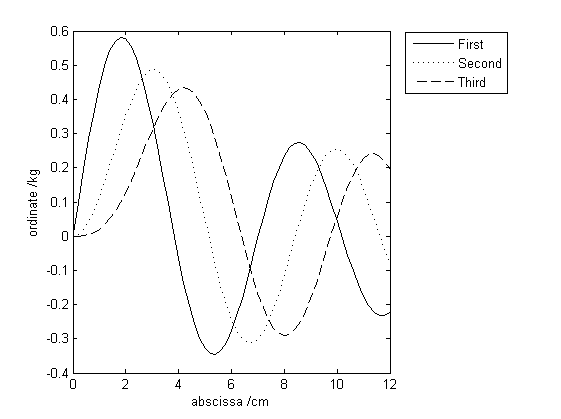
\includegraphics[width=8cm]{fig3.png}
\caption{Lorem ipsum dolor sit amet, consetetur sadipscing elitr, sed diam nonumy eirmod tempor invidunt ut labore et dolore magna aliquyam erat, sed diam voluptua.}
\label{fig:graph}
\end{figure}

\subsection{Equations}
Number equations consecutively with equation numbers in parentheses flush with the right margin, as in (\ref{eq:equation}).
To make your equations more compact, you may use the solidus ($/$), the exp function, or appropriate exponents. Use parentheses to avoid ambiguities in denominators. Punctuate equations when they are part of a sentence, as in 
\begin{equation}
\label{eq:equation}
E = mc^{2}.
\end{equation}
Be sure that the symbols in your equation have been defined before the equation appears or immediately following. Refer to "(\ref{eq:equation})," not "Eq. (1)" or "equation (1)," except at the beginning of a sentence: "Equation (\ref{eq:equation}) is ... ".


%%%%%%%%%%%%%%%%%%%%%%%%%%%%%%%%%%%%%%%%%%%%%%%%%%%%%%%%%%%%%%%%%%%%%%%%%%%%%%%%%%%
% CONCLUSION
\section{Conclusion}
%%%%%%%%%%%%%%%%%%%%%%%%%%%%%%%%%%%%%%%%%%%%%%%%%%%%%%%%%%%%%%%%%%%%%%%%%%%%%%%%%%%
Please note: If your university supervisor is not named as an author, you should change the acknowledgement to: The work has been carried out at Genius Industries, Valley of Innovation and supervised by D. Musterprofessor, Institute of Wisdom, Universität zu Lübeck.


%%%%%%%%%%%%%%%%%%%%%%%%%%%%%%%%%%%%%%%%%%%%%%%%%%%%%%%%%%%%%%%%%%%%%%%%%%%%%%%%%%%
% ACKNOWLEDGEMENT
\section*{Acknowledgement}
%%%%%%%%%%%%%%%%%%%%%%%%%%%%%%%%%%%%%%%%%%%%%%%%%%%%%%%%%%%%%%%%%%%%%%%%%%%%%%%%%%%
The work has been carried out at Genius Industries, Valley of Innovation and supervised by the Institute of Wisdom, Universität zu Lübeck.

As an option, additional acknowledgements can be added.


%%%%%%%%%%%%%%%%%%%%%%%%%%%%%%%%%%%%%%%%%%%%%%%%%%%%%%%%%%%%%%%%%%%%%%%%%%%%%%%%%%%
% BIBLIOGRAPHY: Write list of literature in literature.bib in bibstyleformat (http://www.bibtex.org/)
\bibliographystyle{ieeetr}
%%%%%%%%%%%%%%%%%%%%%%%%%%%%%%%%%%%%%%%%%%%%%%%%%%%%%%%%%%%%%%%%%%%%%%%%%%%%%%%%%%%

% Either use an editor, e.g. Jabref
%\bibliography{literature}

% Or include the bibliography in this document
\begin{thebibliography}{1}

\bibitem{Kopka}
H.~Kopka and P.~W. Daly, \emph{A Guide to \LaTeX}. Addison-Wesley, Harlow, 1999.

\bibitem{BMT}
BMT 2018 Aachen, \emph{Save the Date}. Available: https://www.vde.com/en/events/bmt [last accessed on 2017-11-30].

\bibitem{Young}
M.~Young, \emph{The Technical Writer's Handbook}. University Science, Mill Valley, 1989. 

\bibitem{Kaethner}
C.~Kaethner, J.~M\"uller and T.~M.~Buzug, \emph{Phantom-based Determination of Noise Distribution in Computed Tomography}. In: Student Conference on Medical Engineering Science 2012, Grin Publishing, M\"unchen, pp. 59--62, 2012.

\bibitem{Zongker}
D.~Zongker, \emph{Chicken Chicken Chicken}. Annals of Improbable Research, vol. 12, no. 5, pp. 16--21, 2006.

\end{thebibliography}


\end{document}
%%%%%%%%%%%%%%%%%%%%%%%%%%%%%%%%%%%%%%%%%%%%%%%%%%%%%%%%%%%%%%%%%%%%%%%%%%%%%%%%%%%